\documentclass[a4j,12pt,]{jarticle}
 \usepackage{float}
 \usepackage{siunitx} %%SI単位系用
 \usepackage{amssymb, amsmath}
 \usepackage{ascmac,here,txfonts}
 \usepackage{hyperref}
 \usepackage{listings}
 \usepackage{pxjahyper}
 \usepackage[dvipdfmx]{graphicx}
 \usepackage{amssymb, amsmath}
  \usepackage{listings}
  \usepackage[dvipdfmx]{color}
 
 \lstset{
   language={Python},
   basicstyle={\ttfamily},
   identifierstyle={\small},
   commentstyle={\small\itshape},
   keywordstyle={\small\bfseries},
   ndkeywordstyle={\small},
   stringstyle={\small\ttfamily},
   frame={single},
   breaklines=true,
   columns=[l]{fullflexible},
   numbers=left,
   xrightmargin=0zw,
   xleftmargin=3zw,
   numberstyle={\scriptsize},
   stepnumber=1,
   numbersep=1zw,
   lineskip=-0.5ex,
 }
\begin{document}

{\noindent\small 第13回報告書 \hfill\today}
\begin{center}
  {\Large 太陽光発電システムのシミュレーションと実測データの位相差分析}
\end{center}
\begin{flushright}
  祖父江匠真 \\
\end{flushright}

\section{概要}
今回は, 太陽光発電システムのパフォーマンスをシミュレーションするPblivライブラリを用いて計算した日射量(計算データ)と, リサイクル館に設置した太陽光パネルが受け取った日射量(実測データ)の間の位相差を計算することで実測データの時刻合わせが可能か検証した.

\section{検証方法}
検証には, 図 \ref{p1} に示す2022年4月8日の実測データと, 同じタイムスタンプ列を持つ計算データを使用した.

\begin{figure}[H]
  \begin{center}
    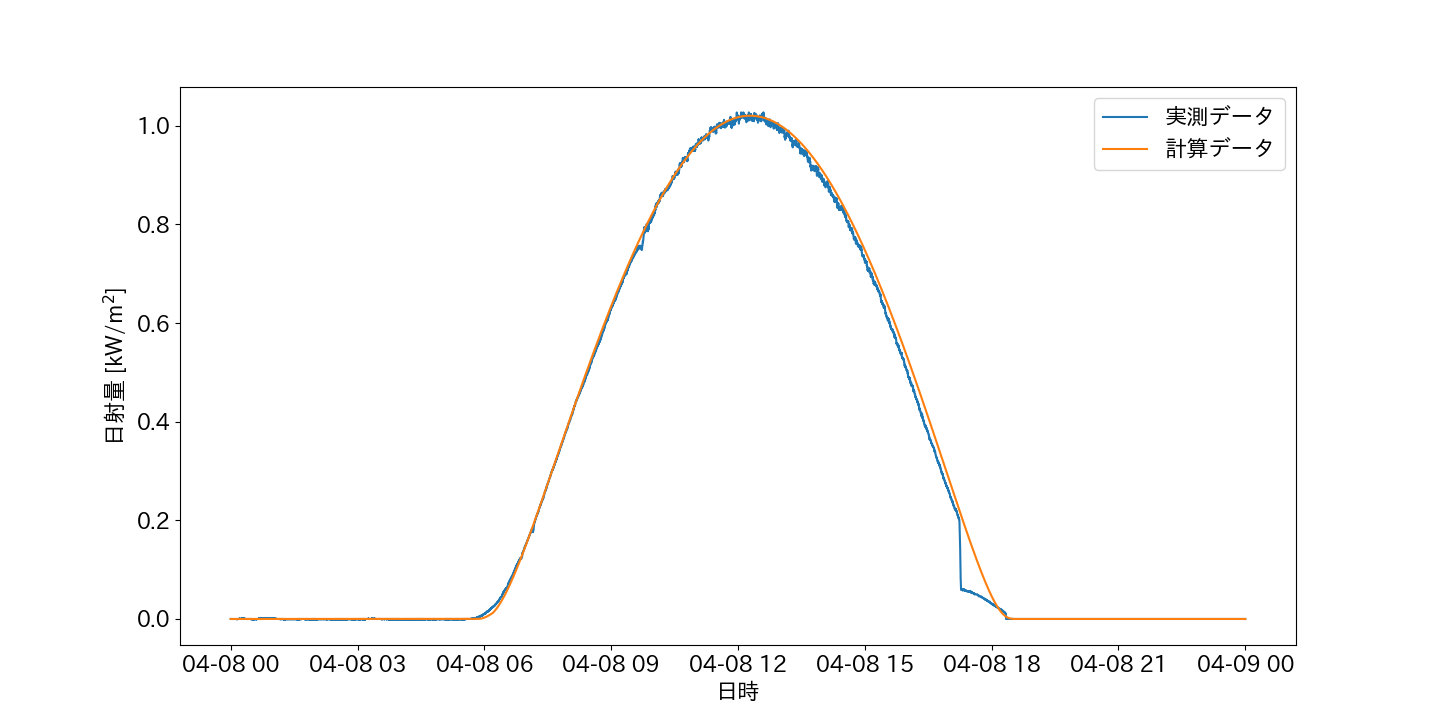
\includegraphics[width=160mm]{real_and_calced.png}
    \caption{検証に使用した実測データと計算データ}
    \label{p1}
  \end{center}
\end{figure}

検証は以下手順で行った.

\begin{enumerate}
  \item scipy.fft.fft メソッドを使用して, 実測データと計算データの高速フーリエ変換(FFT)を行い, 振幅スペクトルを取得する.  
  \item numpy.abs メソッドを使用して, 振幅スペクトルで最も振幅が大きい点に対応する位相を求め, 実測データと計算データの位相差をnumpy.angleメソッドを用いて計算する. 
  \item 計算データの時間軸データ列を numpy.roll 関数を使用して1s遅らせる方向にずらすごとに上記の位相差の計算を繰り返す. 
\end{enumerate}

本検証では, この計算を0sから1000sまでのずれ時間で繰り返し行った. 

\section{結果}
結果として, 図 \ref{p2}に示すグラフが得られた. 横軸がずらした時間の秒数, 縦軸が実測データと計算データの位相差となっている. 図 \ref{p2}から, 2022年4月8日の場合, 実測データと計算データが1sずれることによって約$7.2723 \times 10^{-5} \mathrm{rad}$の位相差が生じることが分かった.

\begin{figure}[H]
  \begin{center}
    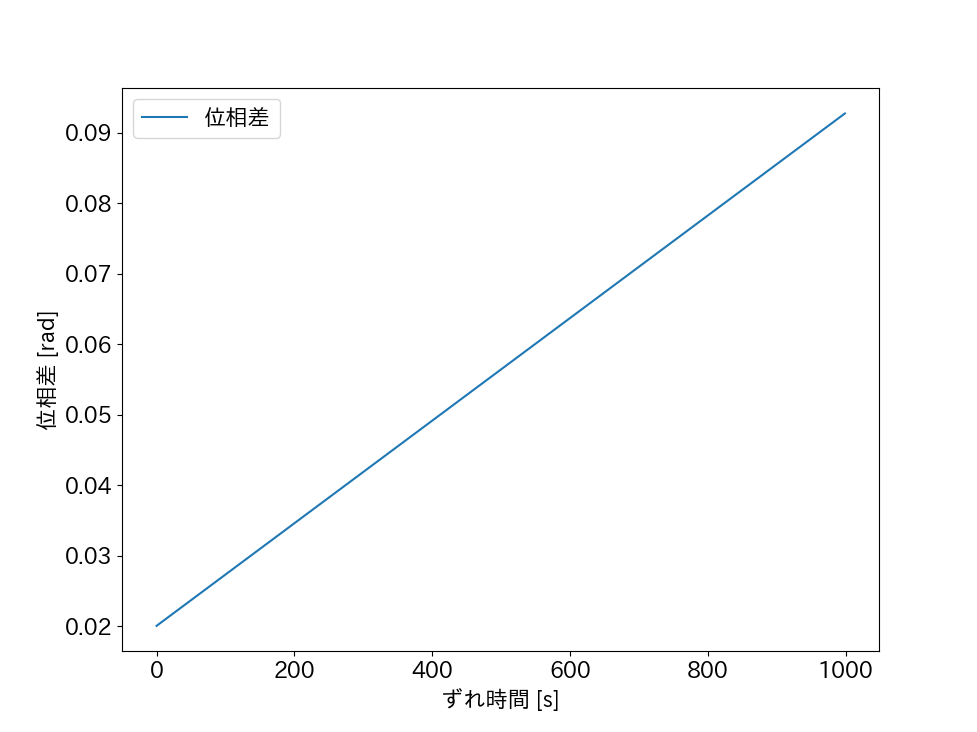
\includegraphics[width=160mm]{1.png}
    \caption{ずれ時間と位相差}
    \label{p2}
  \end{center}
\end{figure}

\section{まとめ}
今回は, Pblivライブラリを用いて計算した日射量データと, リサイクル館に設置した太陽光パネルが受け取った日射量データの間の位相差を計算することで実測データの時刻合わせが可能か検証した.

結果として, 実測データと計算データのずれ時間に対して位相差が線形的に変化することが分かった.

今後は, 位相差を用いた実測データの時刻修正プログラムの開発に取り組む.
\end{document}